\documentclass{hw}
\title{Programming Assignment 4:\\ Intermediate Code Generation}

\usepackage{fancyvrb}
\usepackage{mathpartir}
\usepackage{pervasives}
\usepackage{tikz}
\usetikzlibrary{positioning}

\begin{document}
\maketitle

\section{Metadata}\label{sec:metadata}
% The fully qualified class name of your main program and any other
% instructions needed to run the program.
We implemented programming assignment $1$ and $2$ in Java, but we implemented
programming assignment $3$ and $4$ in OCaml. Our main OCaml executable is
implemented in \texttt{main.ml} inside the \texttt{src} directory. To run our
code, you will need to install a couple of packages and OCaml libraries by
running the following:

\begin{center}
\begin{BVerbatim}
sudo apt-get install aspcud m4 unzip
opam install core async oUnit
\end{BVerbatim}
\end{center}

To build our executable, simply run \texttt{make src}. This will use
\texttt{jflex}, \texttt{cup}, and \texttt{javac} and build all of our Java
code. It will use \texttt{corebuild} to build our OCaml code. Invoking our
code manually is hard; instead, we we recommend you use the \texttt{xic} script
which invokes our code with everything configured properly.

In summary, perform the following:

\begin{center}
\begin{BVerbatim}
sudo apt-get install aspcud m4 unzip
opam install core async oUnit
make src
./xic [flags] <xi_file.xi>...
\end{BVerbatim}
\end{center}

\section{Summary}\label{sec:summary}
In this programming assignment, we implemented intermediate code generation for
the Xi programming language. The most challenging aspect of the assignment was
generating code for complex array operations, including multi-dimensional array
declarations and array concatenation.  This assignment didn't involve many
design decisions; the intermediate representation, code generation algorithm,
lowering algorithm, and block reordering algorithm were all taken from the
notes. Though, we did implement novel forms of testing. There are no known
problems with our implementation.

\section{Specification}\label{sec:specification}
For this project, we have not deviated from the project specification at all.
We have also not implemented any extensions. The spec clarifications we made in
previous assignments still stand.

\section{Design and Implementation}\label{sec:design}
\subsection{Architecture}
\begin{figure}[h]
  \centering
  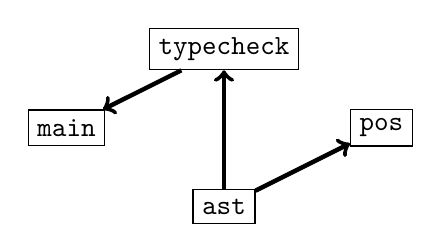
\begin{tikzpicture}
    \tikzstyle{every node}+=[draw]
    \node (main)  at (0, 0)  {\texttt{main}};
    \node (typecheck) at (2, 1)  {\texttt{typecheck}};
    \node (ast)   at (2, -1) {\texttt{ast}};
    \node (pos)   at (4, 0)  {\texttt{pos}};
    \path[->, ultra thick] (ast)   edge (pos)
                           (ast)   edge (typecheck)
                           (typecheck) edge (main);
  \end{tikzpicture}
  \caption{%
    Module Dependency Diagram. Each node represents a module. An arrow from
    module $u$ to module $v$ signifies that $v$ depends on $u$.
  }
  \label{fig:mdd}
\end{figure}

We had four main files in our typechecker, as shown in \figref{mdd}.
\begin{enumerate}
  \item{\texttt{main.ml}:}
    This is the main front end for our compiler. In this class, we handle the
    various command line options passed into the binary and call the rest of
    our lexing, parsing, and typechecking code. We also handle all IO (including the typechecking
    output) in this class.

  \item{\texttt{typecheck.ml}:}
    This file contains the typechecking logic and implements the interface defined by \texttt{typecheck.mli}.

  \item{\texttt{ast.ml}:}
    This file is similar to Ast.java for \texttt{pa2} except that we utilize OCaml. We define our AST nodes by using OCaml abstract data types.

  \item{\texttt{pos.ml}:}
    This class represents a position (row and column) and contains many helpful helper functions that construct expressions and statements without worrying about the position.

\end{enumerate}

\subsection{Code Design and Programming}
\subsubsection{Switch from Java to OCaml}
The most fundamental design decision we made in this project was switching our
main implementation language from Java to OCaml. In our work for PA2,
we found significant overhead in implementing both the AST structure and recursive
traversals over the structure, even with using the Visitor pattern. As an example,
a simple traversal that changed a single field in every AST node took hundreds of lines
of Visitor code. In general, we found an impedance mismatch between the recursive,
immutable style in which we were using our AST and the language we were implementing
it in.

Because of this, we decided at the beginning of our work in PA3 to change to OCaml.
We kept all of our previous lexing and parsing work in Java intact and do all of our
typechecking work in OCaml. To interface between the two languages, we used Jane Street's
S-Expression parser for OCaml: we wrote an S-Expression printer for our AST representation
in Java, the output of which is then parsed into our AST representation in OCaml. On the
whole, we found significant gains in coding speed, code intelligibility and conciseness
due to OCaml features that are particularly well-suited for tree traversals and transformations, such as pattern matching. All four of our group members are also either current or former
CS 3110 TAs, so this made the coding process much more enjoyable for us on the whole.

\subsubsection{OCaml AST}
We followed our practice from Java of annotating AST nodes with an extra type that
stores helpful information (e.g. positions in parsing, types for typechecking). For
maximal flexibility, we designed our OCaml AST such that different types of AST nodes
can be different types. Referring to \texttt{src/ast.ml}, our AST types are polymorphic
in many type parameters to allow for these multifarious annotations. We make use of a
functor to both facilitate the construction of these annotations and for type aliasing.

\subsubsection{Use of the Error monad}
We made significant use of the error monad in all of our typechecking functions. This
allowed us to seamlessly propagate errors throughout our traversals of the AST during
typechecking.

\subsubsection{Jane Street OCaml Core libraries}
We made extensive use of Jane Street's Core libraries, which extend OCaml's standard
library significantly to facilitate everyday programming tasks, such as loading files,
writing files, etc.

\section{Testing}\label{sec:testing}
We sectioned off tests based on the sections highlighted in the Xi Type System Specification - expressions, statements, top-level declarations, and programs. Within each section, we wrote many unit tests that logically and thoroughly verify the types by carefully following the axioms and the typing rules listed in the type specification.

In addition to testing the axioms and typing rules, we created invalid tests to ensure that we are throwing errors on invalid programs, expressions, and statements.

To help make our test cases more readable and cute, we created sexy infix operators, such as \texttt{|-} and \texttt{=:}. A test case \texttt{c |- e =: t} represents a context \texttt{c} that derives the expression \texttt{e} of type \texttt{t}. We also created an infix operator \texttt{=/=} that ensures an error is thrown. For example, \texttt{c =/= e} means that the expression \texttt{e} is ill-typed in the context \texttt{c}. We similarly implemented these operators for statements, callables, and programs.

Our test plan worked out very well. Methodically and meticulously testing our code allowed us to catch many simple oversights before running the test harness provided by the staff.

\section{Work Plan}\label{sec:workplan}
One day during compiler lectures Michael and Ralph had an enlightenment -- switching our
source language from Java to OCaml.
They slowly approached Seung Hee and Alice after class and they didn't know at the moment,
but they were about to embark on the most incredible journey of their life. After discussing
with professor Myers, we decided to go with the idea. Ralph and Michael immediately
worked on the conversion from Java to OCaml. Then after the skeleton of OCaml code was written
we split up the work. Ralph worked on type checking expressions, Michael on statements,
and Seung Hee and Alice pair programmed on type checking functions. Then, while
Ralph worked on the front end, Seung Hee, Michael and Alice focued on testing.

\section{Known Problems}\label{sec:problems}
Currently we do not support UTF-8 as OCaml does not have good support for unicode
escapes.

\section{Comments}\label{sec:comments}
We spent about 80 hours total on the assignment. The assignment overall
introduced important concepts about type checking. We really appreciated
the type checking specification. It was very thorough and the case analysis
really helped structure our code.

\end{document}
